\section{Model Formulation and Solution for Problem 2}

\subsection{Model Formulation}

Problem 2 reoptimizes execution regions and start times using actual jobs and hourly electricity parameters for hours 0--2399; forecasts do not enter scheduling. Hours 2400--2405 are reserved for completion and settlement, and all jobs must finish before 2406. Storage is excluded.
Research on carbon-aware data centers identifies grid carbon intensity as an important signal for job scheduling and energy management\cite{ref5}.
Cross-region load shifting exploits regional differences in electricity and carbon conditions,
but introduces network latency and service-quality costs\cite{ref6}.
Accordingly, we evaluate cost, emissions, communication latency, and renewable utilization subject to deadlines, latency, GPU, and power constraints.

Job parameters and fractional hourly occupancy follow Problem 1. Real-time jobs start immediately, while flexible jobs may shift within their valid time windows.
Let $x_{irs}$ indicate whether job $i$ starts in region $r$ at time $s$.
Candidate regions $R_i$ satisfy network latency limits,
and candidate start times $S_i$ satisfy arrival, completion, and terminal constraints at 2406.

The AI IT load, total IT load, and facility load in region $r$ at time $t$ are denoted by
$P^{AI}_{rt}$, $P^{IT}_{rt}$, and $F_{rt}$, respectively.
Using fractional occupancy from Equation~(\ref{eq:q1_overlap}),
\begin{equation}
	\begin{aligned}
		P^{AI}_{rt}
		&=
		\sum_i\sum_{s\in S_i}
		p_i\rho_{ist}x_{irs},\\
		P^{IT}_{rt}
		&=
		P^{NonAI}_{rt}+P^{AI}_{rt},\\
		F_{rt}
		&=
		PUE_rP^{IT}_{rt}.
	\end{aligned}
	\label{eq:q2_load_mapping}
\end{equation}

Hourly GPU occupancy retains the Problem 1 constraints. IT capacity, facility capacity, and maximum grid purchase capacity define an effective AI IT limit
$\bar P^{AI}_{rt}
=\min\{P^{IT,\max}_{rt}-P^{NonAI}_{rt},
P^{Facility,\max}_{rt}/PUE_r-P^{NonAI}_{rt},
(P^{RE}_{rt}+P_r^{Grid,\max})/PUE_r-P^{NonAI}_{rt}\}$,
with $P^{AI}_{rt}\leq\bar P^{AI}_{rt}$; GPU, latency, and deadline constraints otherwise follow Problem 1.

Without storage, renewables first serve local loads. Grid purchases cover any deficit, exports use available surplus up to the export limit, and the remainder is curtailed.
Let $V_{rt}$, $B_{rt}$, $X_{rt}$, and $R_{rt}$ denote
direct renewable use, grid purchases, renewable exports, and curtailment, respectively. Then
\begin{equation}
	\begin{aligned}
		V_{rt}&=\min(F_{rt},P^{RE}_{rt}),\\
		B_{rt}&=\max(F_{rt}-P^{RE}_{rt},0),\\
		X_{rt}&=\min\{\max(P^{RE}_{rt}-F_{rt},0),\bar X_r\},\\
		R_{rt}&=P^{RE}_{rt}-V_{rt}-X_{rt},
	\end{aligned}
	\label{eq:q2_energy}
\end{equation}
Here $0\leq B_{rt}\leq P_r^{Grid,\max}$ and $0\leq X_{rt}\leq\bar X_r$.

The schedule is evaluated using net operating cost $C$, carbon emissions $E$, average network latency $L$,
and renewable utilization $U$.
For $t=0,\ldots,2405$, define
\begin{equation}
	\begin{aligned}
		C
		&=
		\sum_r\sum_{t=0}^{2405}
		\left(\pi_{rt}B_{rt}-\sigma_{rt}X_{rt}\right),\\
		E
		&=
		\sum_r\sum_{t=0}^{2405}\kappa_{rt}B_{rt},\\
		L
		&=
		\frac{1}{N}
		\sum_i\sum_{r\in R_i}\sum_{s\in S_i}
		l_{ir}x_{irs},\\
		U
		&=
		\frac{\displaystyle
			\sum_r\sum_{t=0}^{2405}(V_{rt}+X_{rt})}
		{\displaystyle
			\sum_r\sum_{t=0}^{2405}P^{RE}_{rt}},
		\qquad Q=1-U.
	\end{aligned}
	\label{eq:q2_objectives}
\end{equation}

Let $f_1=C,f_2=E,f_3=L,f_4=Q$. Single-objective continuous relaxations yield ideal lower bounds $f_m^{LB}$. Together with the computing-only baseline $f_m^0$ and single-objective anchors $x^{(a)}$, these define fixed normalization scales:
\begin{equation}
	\begin{aligned}
		f_m^{ref}
		&=
		\max\left\{
		f_m^0,\max_a f_m(x^{(a)})
		\right\},\\
		R_m
		&=
		f_m^{ref}-f_m^{LB},\\
		d_m(x)
		&=
		\frac{f_m(x)-f_m^{LB}}{R_m},\\
		\min\quad z,
		&\qquad d_m(x)\leq z,\quad \forall m .
	\end{aligned}
	\label{eq:q2_minmax}
\end{equation}

If $R_m\approx0$, the metric is used only for evaluation; otherwise Equation~(\ref{eq:q2_minmax}) minimizes the maximum normalized deviation.

Multiscale rolling optimization handles dynamic coupling among job arrivals, loads, and energy states\cite{ref7}; low-carbon online scheduling must also coordinate service quality and energy metrics\cite{ref8}. For 50000 jobs, we use a decision window of $H=24$ h and a look-ahead window of $K=48$ h, with feasibility repair and local mixed-integer linear programming refinement.
At rolling origin $\tau$,
we examine $[\tau,\tau+H+K)$,
but commit only jobs actually starting within $[\tau,\tau+H)$.
Already started jobs retain their existing schedules;
flexible jobs whose latest valid start enters the current window must start in this iteration.

The construction phase schedules real-time jobs first, then sorts flexible jobs by time slack and resource demand.
Define the current full-horizon objective estimate as
$\hat f_{m,\tau}
=f_m^0+\Delta f_{m,\tau}^{past}
+f_{m,\tau}^{scope}-f_{m,\tau}^{0,scope}$.
For each valid candidate $(r,s)$, compute
\begin{equation}
	S_{irs}
	=
	\max_m
	\left\{
	\frac{
		\hat f_{m,\tau}
		+\Delta f_{m,irs}
		-f_m^{LB}}
	{R_m}
	\right\},
	\qquad
	(r_i^*,s_i^*)
	=
	\arg\min_{(r,s)}S_{irs}.
	\label{eq:q2_marginal}
\end{equation}

Capacity conflicts trigger rescheduling of replaceable jobs. Once feasible, key jobs form a large neighborhood, and refinement fixes decisions outside that neighborhood. Table~\ref{tab:q2_algorithm} summarizes the procedure.

\begin{table}[H]
	\centering
    \caption{Rolling matheuristic for Problem 2}
	\label{tab:q2_algorithm}

	\fontsize{10.5pt}{12pt}\selectfont
	\renewcommand{\arraystretch}{0.88}

	\begin{tabular}{
			>{\centering\arraybackslash}p{0.08\textwidth}
			>{\raggedright\arraybackslash}p{0.86\textwidth}}
		\toprule
        \textbf{Step} & \multicolumn{1}{c}{\textbf{Operation}}\\
		\midrule

		1 &
        Determine fixed normalization scales from continuous relaxations, the Problem 2 computing-only baseline, and single-objective anchors.\\

		2 &
        Read the $H=24$ h decision window and $K=48$ h look-ahead interval;
        lock already started jobs and identify jobs required to start now.\\

		3 &
        Schedule real-time jobs immediately; sort flexible jobs by slack and resource demand,
        then use Equation~(\ref{eq:q2_marginal}) to select feasible candidates.\\

		4 &
        Update GPU occupancy, AI IT loads, and energy states;
        reschedule replaceable jobs when capacity conflicts occur.\\

		5 &
        Select key jobs to form a large neighborhood,
        fix decisions outside it, and refine using a small mixed-integer linear program.\\

		6 &
        Commit the current $H$-hour decisions and continue rolling;
        finally reconstruct the full profile for hours 0--2405 and verify it independently.\\

		\bottomrule
	\end{tabular}
\end{table}


Candidates are evaluated by the original multiobjective criterion; the matheuristic only restricts the integer search space. It produces computationally efficient feasible schedules satisfying all hard constraints; global optimality is not claimed.


\subsection{Results and Model Validation}

A full-horizon computing-only baseline for 50000 jobs follows the Problem 1 principles and is settled under Problem 2 energy accounting. Table~\ref{tab:q2_result} gives rolling optimization results.

\begin{table}[H]
	\centering
    \caption{Problem 2 multiobjective schedule versus its computing-only baseline}
	\label{tab:q2_result}

	\fontsize{10.5pt}{12pt}\selectfont
	\renewcommand{\arraystretch}{0.90}

	\begin{tabular}{lccc}
		\toprule
        \multicolumn{1}{c}{\textbf{Metric}}
        & \textbf{Computing baseline}
        & \textbf{Balanced schedule}
        & \textbf{Change}\\
		\midrule

        Net cost/CNY
		& $-4.196834\times10^8$
		& $-4.247568\times10^8$
        & $-507.34$ (CNY $10^4$)\\

        Emissions/tCO$_2$
		& 8.850562
		& 10.125791
        & $+1.275228$\\

        Mean latency/ms
		& 5.000000
		& 12.946840
        & $+7.946840$\\

        Renewable utilization
		& 67.91598\%
		& 68.13914\%
        & $+0.22316$ pp\\

        Mean waiting/h
		& 0.00116
		& 30.89284
        & $+30.89168$\\

        Migration share
		& 0
		& 29.35800\%
        & $+29.35800$ pp\\

		\bottomrule
	\end{tabular}
\end{table}


Table~\ref{tab:q2_result} shows a net cost reduction of 507.34 units of CNY $10^4$ and a renewable utilization increase of 0.22316 percentage points, alongside emission and mean latency increases of 1.2752 tCO$_2$ and 7.95 ms. Negative cost means export revenue exceeds electricity purchase expenditure.

With fixed normalization, the four deviations are 1.00, 1.00, 0, and 1.00 for the computing baseline, versus 0.85, 1.14, 1.15, and 0.87 for the Problem 2 schedule, giving a maximum deviation $z=1.15$.

\begin{figure}[H]
	\centering
	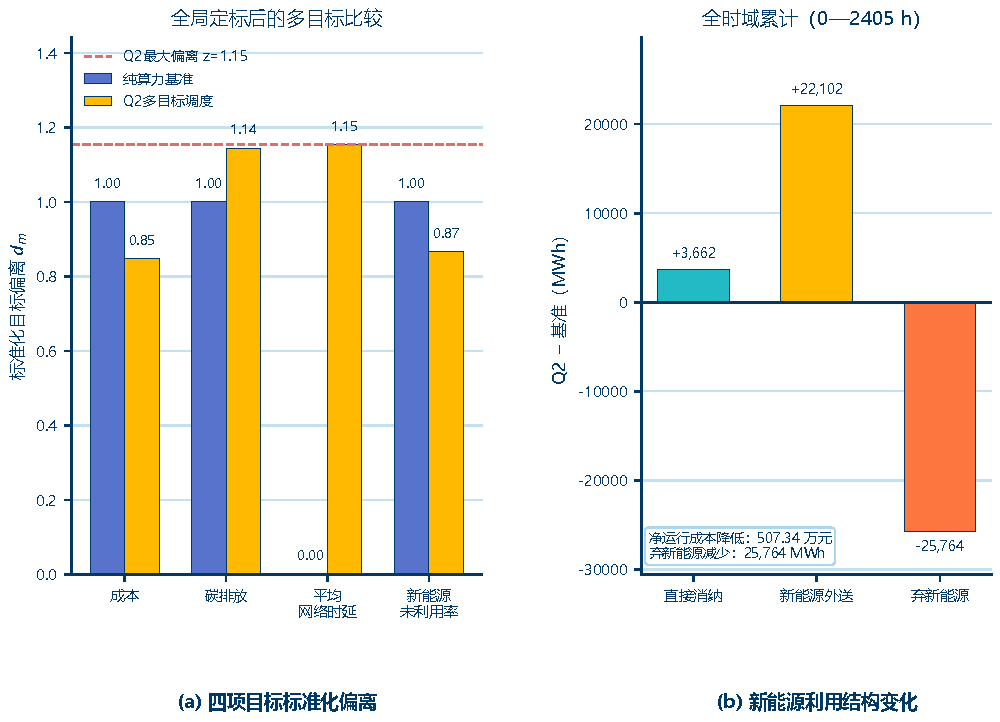
\includegraphics[width=0.82\textwidth]
	{figures/q2_group1_core_results.pdf}
    \caption{Problem 2 multiobjective results and changes in renewable utilization}
	\label{fig:q2_core}
\end{figure}

In Figure~\ref{fig:q2_core}, direct renewable use and exports increase by approximately 3662 and 22102 MWh, respectively, while curtailment falls by about 25764 MWh. These changes approximately balance.

Of all jobs, 35321 execute locally and 14679 migrate across regions. The migration share is 29.358\%, with migrated work of $1.308142\times10^6\,\mathrm{GPU\cdot h}$.

Figure~\ref{fig:q2_migration} shows more outward migration from D, E, and F, with C and D absorbing more cross-region computing work. Both resource and energy conditions influence migration directions.

Reconstructed profiles for hours 0--2405 from all 50000 job records preserve cumulative quantities in both schedules: AI IT energy is $7.389279853\times10^5$ MWh and GPU work is $5.020787\times10^6$ GPU$\cdot$h.
There are no job, latency, deadline, capacity, or grid purchase violations. Energy balance residuals are zero, and no job occupies resources at 2406.

Of 91 refinement windows, 45 accept improvements, with a mean improvement of 2.43\%. Exact comparisons for windows 0--9 give a median speedup of approximately 31.8, a mean absolute relative deviation of 39.82\%, and a maximum normalized-objective deviation of 293.40\%. The maximum is a relative deviation of the local-window normalized objective, not a full-horizon error in cost or emissions. However, it shows that restricted neighborhoods can miss better job combinations in some resource-constrained windows. We therefore describe the method only as a large-scale approximation satisfying all hard constraints, without claiming local or full-horizon optimality.

\begin{figure}[H]
	\centering
	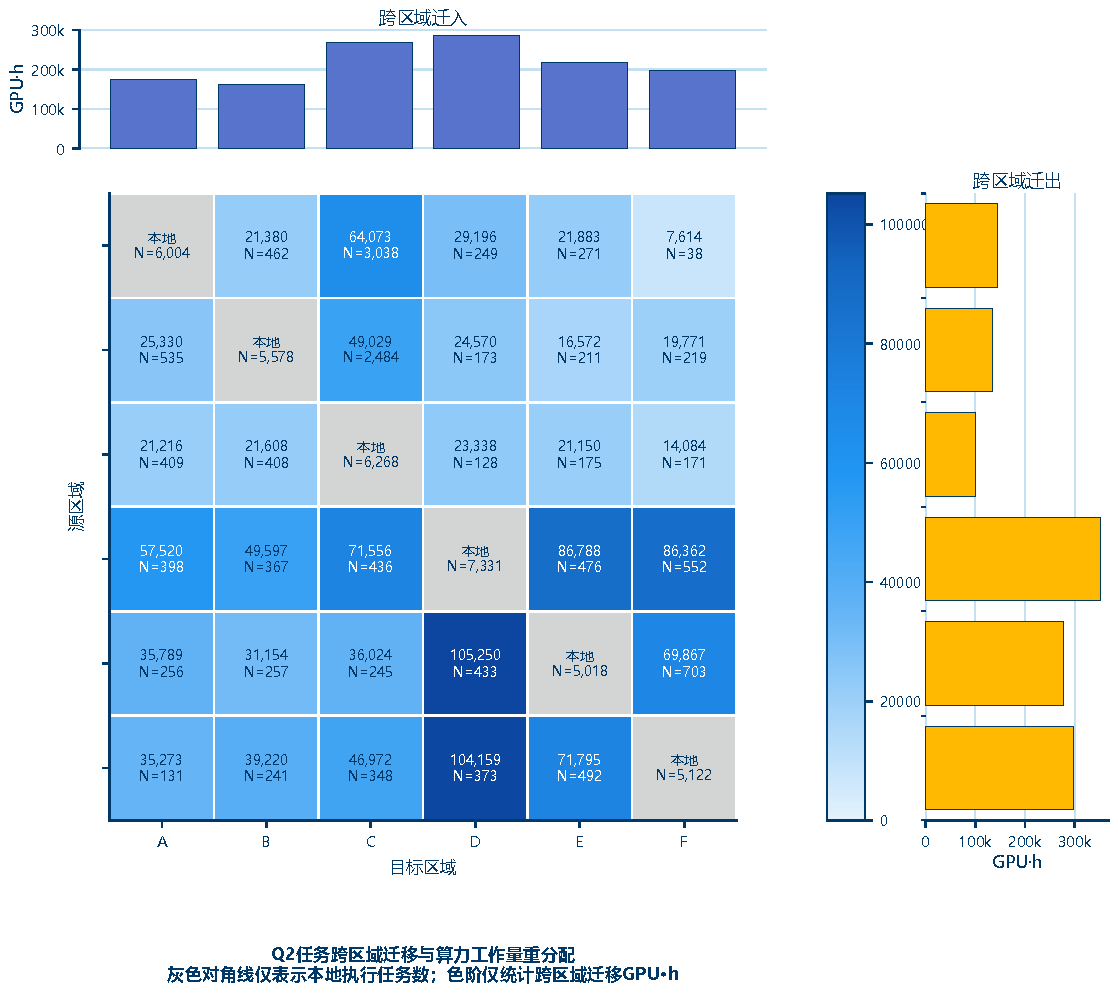
\includegraphics[width=0.68\textwidth]
	{figures/q2_group2_dispatch_mechanism.pdf}
    \caption{Cross-region job migration and computing-work redistribution in Problem 2}
	\label{fig:q2_migration}
\end{figure}

\begin{figure}[H]
	\centering
	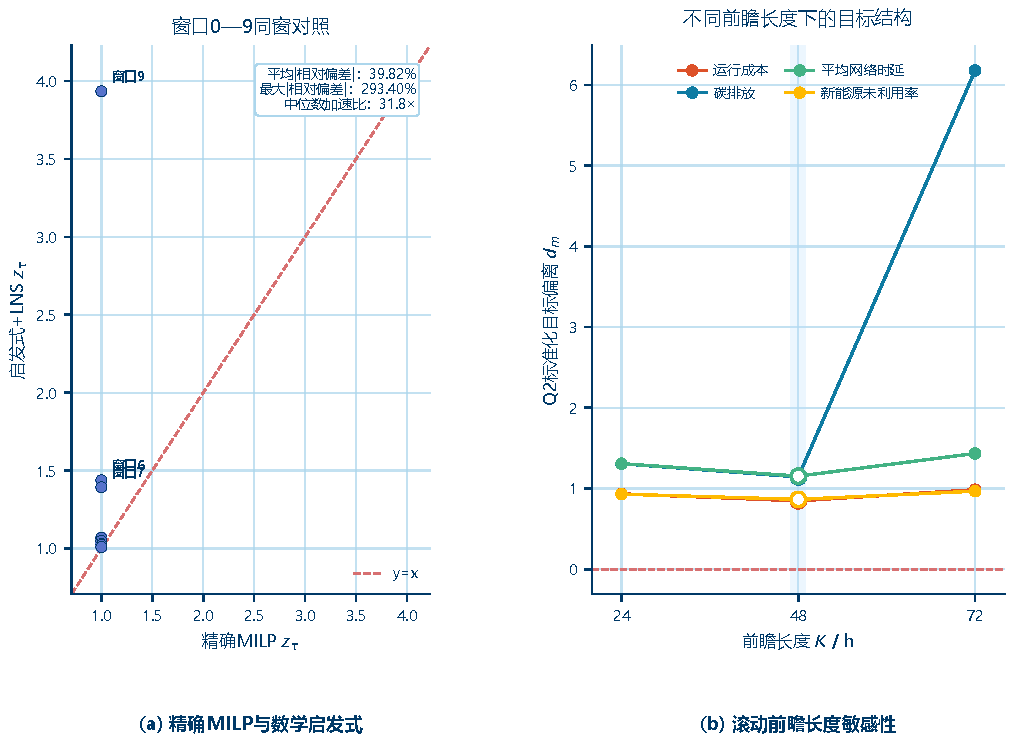
\includegraphics[width=0.72\textwidth]
	{figures/q2_group3_model_validation.pdf}
    \caption{Problem 2 matheuristic quality and look-ahead sensitivity}
	\label{fig:q2_validation}
\end{figure}

Look-ahead tests show similar objective structures at $K=24$ h and 48 h, while $K=72$ h only substantially raises emissions. We therefore use $H=24$ h and $K=48$ h.

Problem 2 exchanges higher emissions, latency, and waiting for lower cost and better renewable utilization. Independent full-horizon recomputation confirms hard-constraint compliance, allowing this schedule to initialize the job side of Problem 4.
